Our novel graph-based approach to model the dynamics of the agents' health states incorporates communal effects and temporal decease effects through a graph contribution and an individual health contribution term, respectively.

Our main propagation rule is based on the definition of a graph convolution shown in Eq.~\eqref{eq:graph_convolution} and reads as follows in component notation
\begin{equation}
	\label{eq:state_propagation}
	h_{v_i, m}^{(l+1)}
	=
	\underbrace{
		\sum_k \frac{\hat{A}_{v_i, k}^{(l)}}{\sum_j \hat{A}_{v_i, j}^{(l)}} h_{k, m}^{(l)} \delta_{m, 1}
	}_{\text{\textcolor{red}{Graph}}}
	+
	\underbrace{
		{(h_{v_i}^{(l)}\cdot T)}_m
	}_{\text{\textcolor{blue}{Temporal}}}
\end{equation}
with $m$ being the health state index ranging from $0$ to $2$, $\hat{A}_{v_i, k}^{(l)}$ infection-adjusted adjacency matrix component, $\delta$ the Kronecker delta and $T$ as temporal transition matrix.

The propagation consists of two parts, first the graph contribution and second the temporal contribution. While the former captures the dynamics of infections based on the social contacts between agents, the former ensures that an infected agent heals over time and becomes resistant against the Corona virus. Figure~\ref{fig:state_propagation} visualises the propagation rule and the two subsequent sections explain the terms in greater detail.

\begin{figure}[H]
	\centering
	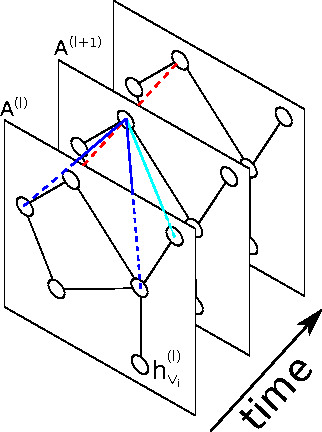
\includegraphics[width=0.8\columnwidth]{img/state_propagation.pdf}
	\caption{Visualisation of propagation rule from equation~\eqref{eq:state_propagation}. The blue connection visualises the temporal term and the red connections visualise the graph term. The dashed red line is does not contribute to the graph term as the two nodes are not connected according to $\hat{A}(l)$.}
	\label{fig:state_propagation}
\end{figure}

\subsection{Explanation of the graph contribution term}

The graph contribution models how infected agents spread the disease through contacts with susceptible agents. This is modeled by the term

\begin{equation}
	(h_{v_i, m}^{(l+1)})_{\text{Graph}} = \sum_k \textcolor{cyan}{\frac{\hat{A}_{v_i, k}^{(l)}}{\sum_j \hat{A}_{v_i, j}^{(l)}}} h_{k, m}^{(l)} \textcolor{orange}{\delta_{m, 1}}.
\end{equation}

A sum over all neighbouring agents' features $h_{k,m}^{(l)}$ is weighted by the normalised infection-adjusted graph connections as shown in cyan. The Kronecker delta, as shown in orange, ensures that only the I feature is added as this is the only one that matters during social contacts between agents.

The infection-adjusted adjacency matrix $\hat{A}$ is constructed from $A$ and $I$ which are the regular continuous adjacency matrix and the infection matrix, respectively. These three quantities are explained in the following:
	
\begin{itemize}
	\item The adjacency matrix $A$ is time dependent, $A^{(l)}$, and inferred from data. In our use case, $A_{ij} = \frac{1}{dist(v_i, v_j)+\epsilon}$, hence $A_{ij}$ is large when persons $i$ and $j$ have been in contact. $\epsilon$ serves as regularization for small distances.
	\item The infection matrix is constructed as
	\begin{equation}
	I =
	\begin{pmatrix}
	0     &  0  & 0 \\
	\beta &  0  & \alpha \\
	0     &  0  & 0
	\end{pmatrix}
	=
	(I_{ij})_{i,j}
	\end{equation}
	with $i$ as the index of the host state and $j$ is the index of the contact person state. The states that we consider here are ordered as follows: susceptible, infected, recovered. $\beta$ denotes the probability of infection  after contact (also known as attack rate). $\alpha$ models the probability of being reinfected, which we assume to be zero ($\alpha=0$) based upon current medical~\cite{Bao2020.03.13.990226}.
	\item $\hat{A}$, with $\hat{A}_{ij}\in [0, 1]$, is the infection-adjusted adjacency matrix that takes the infection interactions into account and is computed as follows
	\begin{equation}
	\hat{A}_{ij} = A_{ij}\cdot \frac{ h_{v_1}^T I h_{v_2} + h_{v_2}^T I h_{v_1} }{\beta}.
	\end{equation}
	The weighted scalar product of the health states of agents $i$ and $j$ is used to evaluate whether the edge is relevant for the infection dynamics. Only when an infected person and a susceptible have contact, the edge $A_{ij}$ should be considered, otherwise it should be dropped.	The sum in the denominator comes from the fact that both, agent $i$ and $j$, can act as host during a contact. The division by $\beta$ normalises the factor to one to ensure $\hat{A}_{ij} \in [0, 1]$. Since $I$ is not symmetric, $p_a$ is a proper normalization because the sum is in $\{0, p_a\}$. Note that the fraction has the desired properties for pure $S$-, $I$- and $R$-persons.
\end{itemize}

Figure~\ref{fig:state_propagation} visualises the influence of the infection-adjusted adjacency matrix to the agents' states at the next time step. The two solid red lines contribute directly while the dashed red lines does not.

\subsubsection{Explanation of the temporal contribution term}

The transition of a person's health state $h_{v_i}^{(l)}$ is determined by three rules that are stated in the following:

\begin{itemize}
	\item A susceptible person always stays susceptible.
	\item An infected person has a probability $\gamma$, called recovery rate, to recover. The complementary probability $1-\gamma$ denotes that the person remains sick.
	\item A recovered person could have a probability to be re-infected, but we assume this to be zero throughout this work. Thus a recovered person always stays recovered~\cite{Bao2020.03.13.990226}.
\end{itemize}

These three rules are combined into a temporal transition matrix $T$, which describes the health state of an agent as time passes. This matrix reads as

\begin{equation}
	T = 
	\begin{pmatrix}
		1 &     0    & 0      \\
		0 & 1-\gamma & \gamma \\
		0 &     0    & 1      \\
	\end{pmatrix}.
\end{equation}

The temporal update rule based on the health status thus becomes

\begin{equation}
	H^{(l+1)} = H^{(l)} T.
\end{equation}